% !TeX root = main.tex

\chapter{Requirements Analysis and Global Design}


% ─────────────────────────────────────────────
\section*{Introduction}
\addcontentsline{toc}{section}{Introduction}
% ─────────────────────────────────────────────

\paragraph{}With the project context and problem statement established in
the previous chapter, this chapter moves into the analysis and design phase.
We begin by presenting the Agile Scrum methodology adopted to structure the
work across the internship period. We then examine existing tools that
address similar problems and explain why none of them were suitable for this
specific context. From there, we derive the functional and non-functional
requirements the system must satisfy, translate them into a global
architecture, and present the product backlog and sprint plan that guided
the implementation. The chapter closes with a description of the technical
environment used throughout the project.


% ─────────────────────────────────────────────
\section{Development Methodology}
% ─────────────────────────────────────────────

\paragraph{}Since the QA team are the primary users of this application, their feedback was essential at every stage of the development process, so they could review the delivered features and provide concrete feedback on what needed to be improved, removed, or added. This close and continuous collaboration made Agile the best choice, as it is built around short delivery cycles that end with a review, allowing the product to be shaped progressively based on real user input. Among the available Agile frameworks, Scrum was selected for its simple structure, its defined feedback points at the end of each sprint, and its ability to incorporate changes without disrupting the overall plan \cite{schwaber2020scrum}.


% ─────────────────────────────────────────────
\subsection{Scrum Framework Overview}
% ─────────────────────────────────────────────

\paragraph{}Scrum organizes work into fixed-length iterations called
\textbf{sprints}, each ending with a potentially shippable increment of the
product. Three core roles structure the team, three artifacts capture the
work, and four ceremonies punctuate each sprint cycle, as illustrated in
Figure~\ref{fig:scrum}.

\begin{figure}[H]
\centering
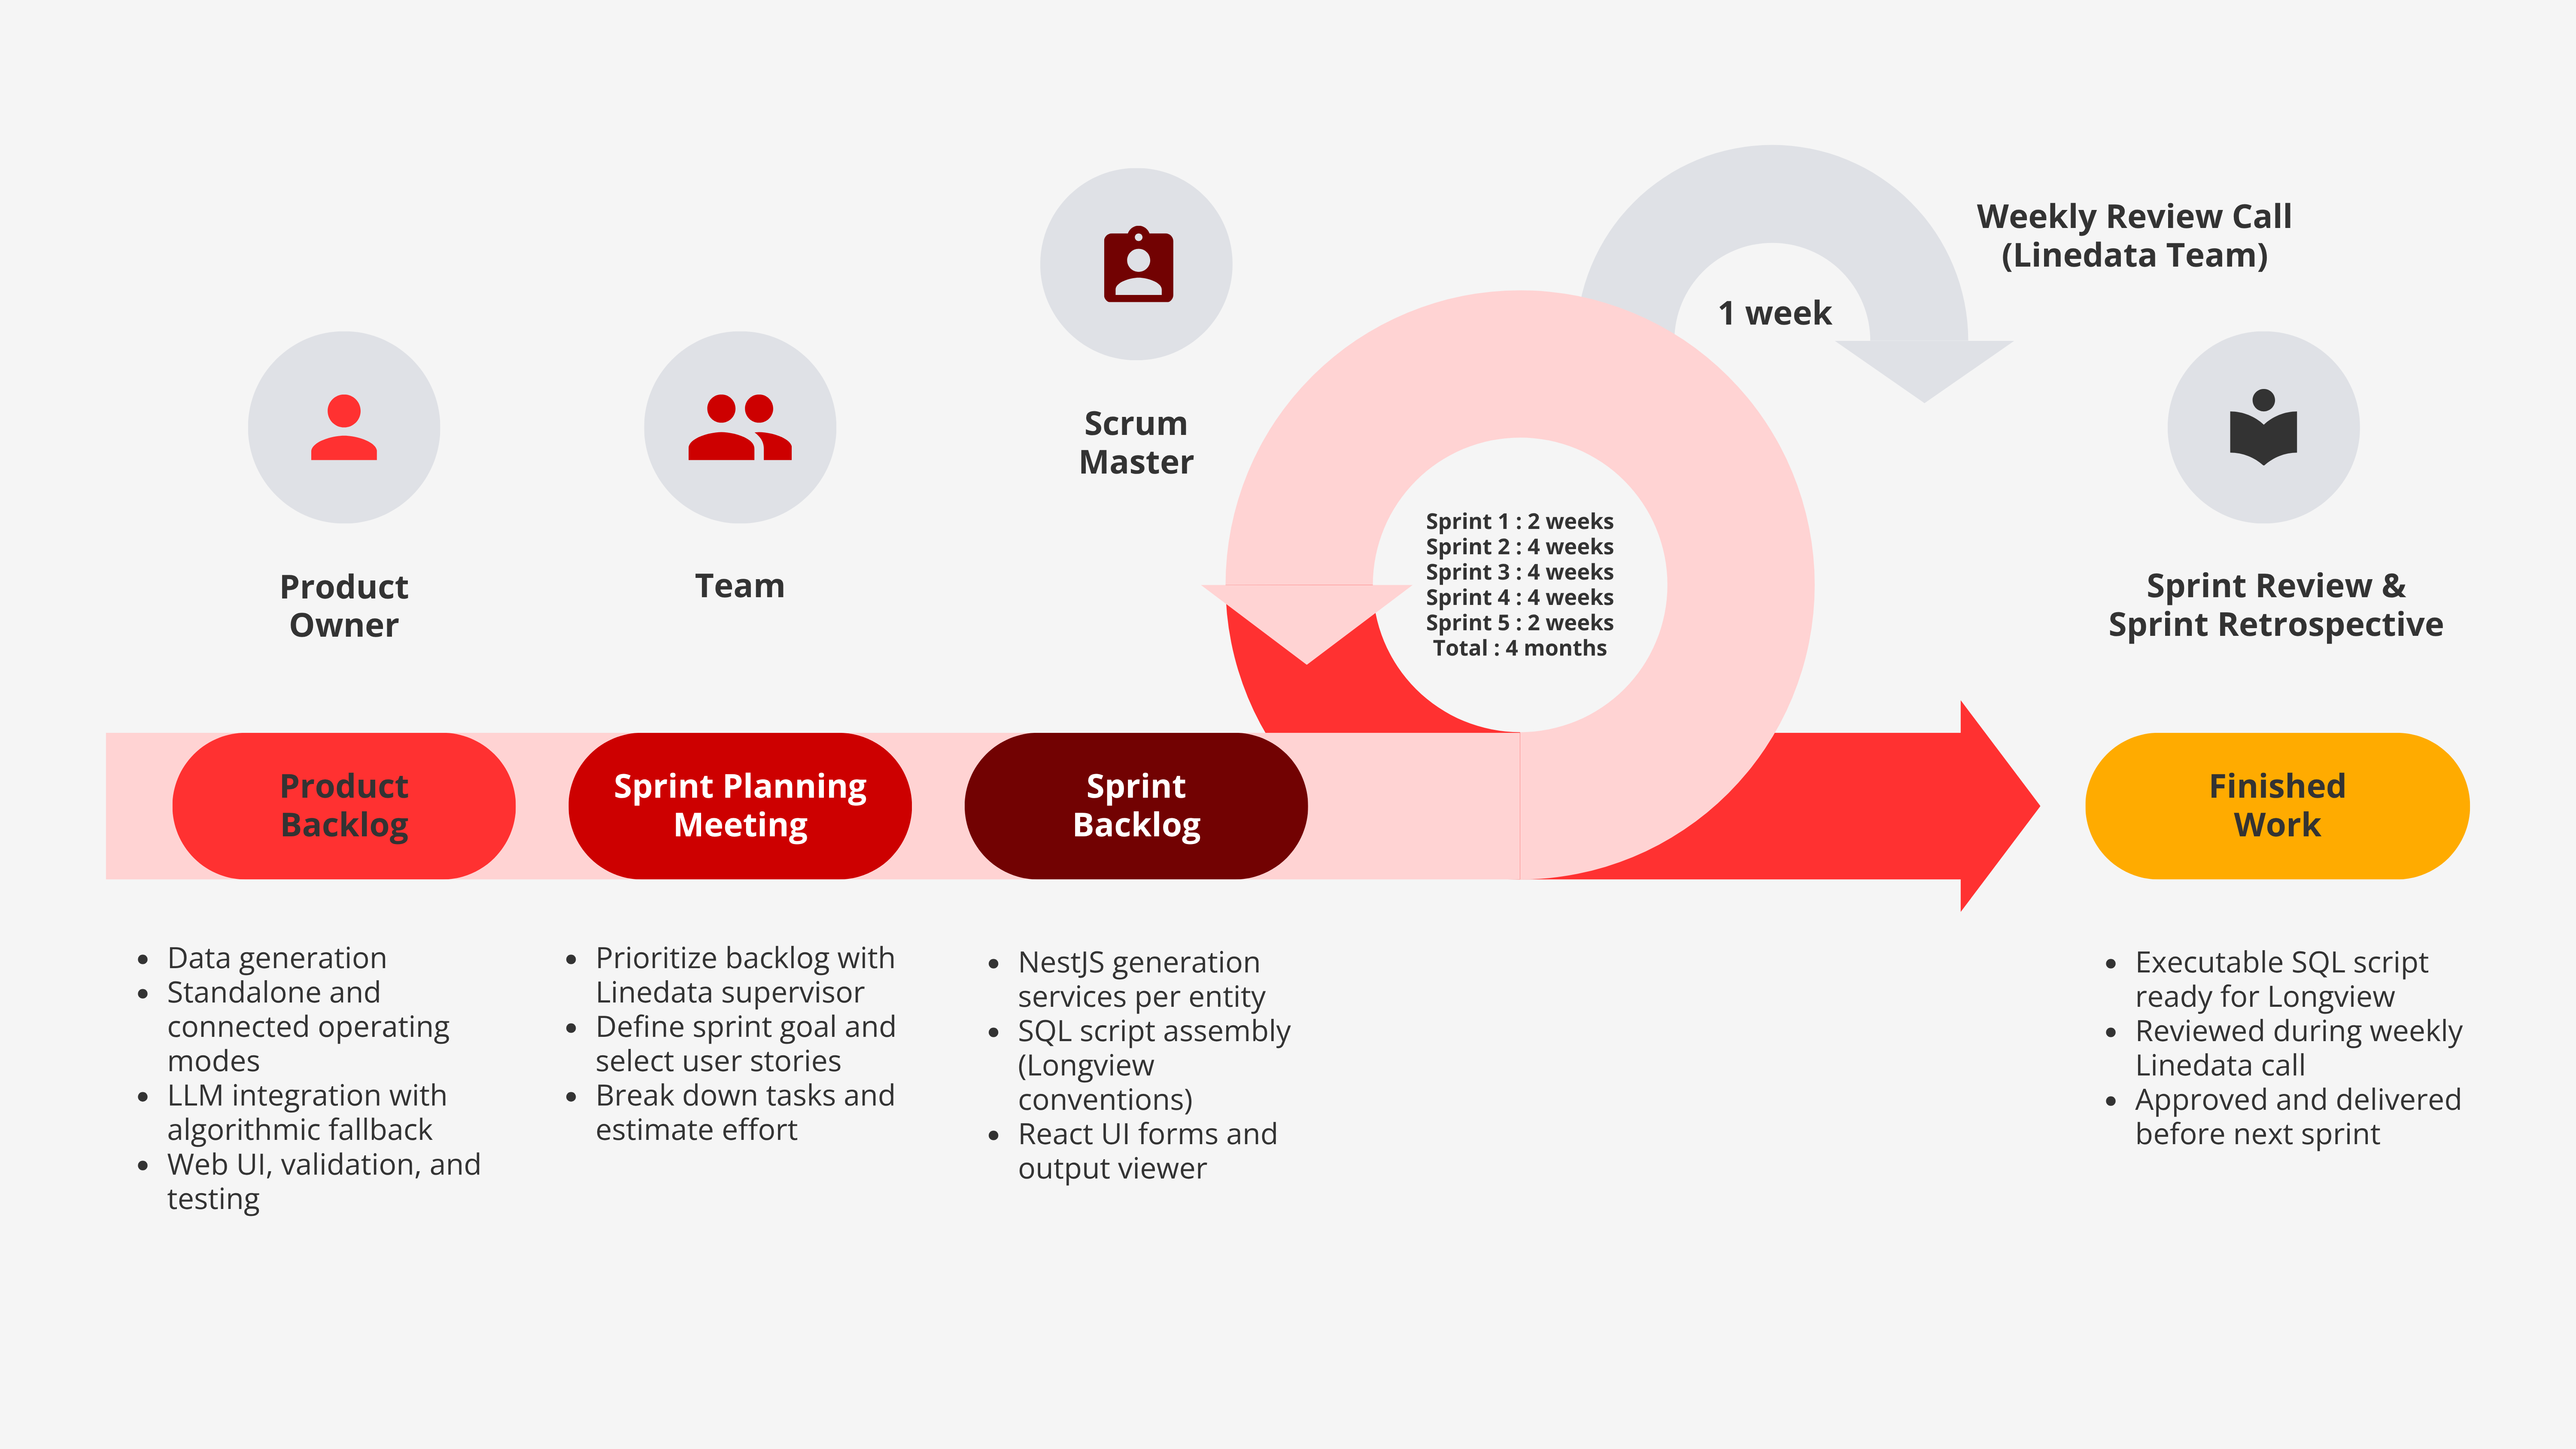
\includegraphics[width=0.85\textwidth]{img/scrum-process.png}
\caption{The Scrum process framework}\label{fig:scrum}
\end{figure}

\paragraph{}Within this project, the Scrum roles were adapted to the
internship context as follows:

\begin{itemize}
    \item \textbf{Product Owner:} The internship supervisor at Linedata,
    responsible for defining priorities, validating deliverables, and
    ensuring the tool aligned with the team's actual testing needs.
    \item \textbf{Scrum Master / Developer:} The intern, responsible for
    planning, executing, and delivering each sprint increment, managing
    impediments, and adjusting scope when needed.
\end{itemize}

\paragraph{}The Scrum artifacts and ceremonies were applied as follows:

\begin{itemize}
    \item \textbf{Product Backlog:} A prioritized list of all features and
    tasks to be delivered across the project lifetime.
    \item \textbf{Sprint Backlog:} The subset of backlog items committed to
    for each sprint, refined at the start of each cycle.
    \item \textbf{Sprint Increment:} The functional, testable deliverable
    produced at the end of each sprint, demonstrated to the supervisor
    during the sprint review.
    \item \textbf{Weekly Review Call:} Given the internship context,
    the classical daily stand-up was replaced by a weekly call with
    the Linedata development team, during which progress was demonstrated,
    feedback was collected, and priorities for the coming week were adjusted.
\end{itemize}


% ─────────────────────────────────────────────
\subsection{Sprint Planning Overview}
% ─────────────────────────────────────────────

\paragraph{}The internship was organized into five sprints, each targeting
a distinct phase of the project. Figure~\ref{fig:sprint-plan} gives an
overview of the sprint plan.

\begin{figure}[H]
\centering
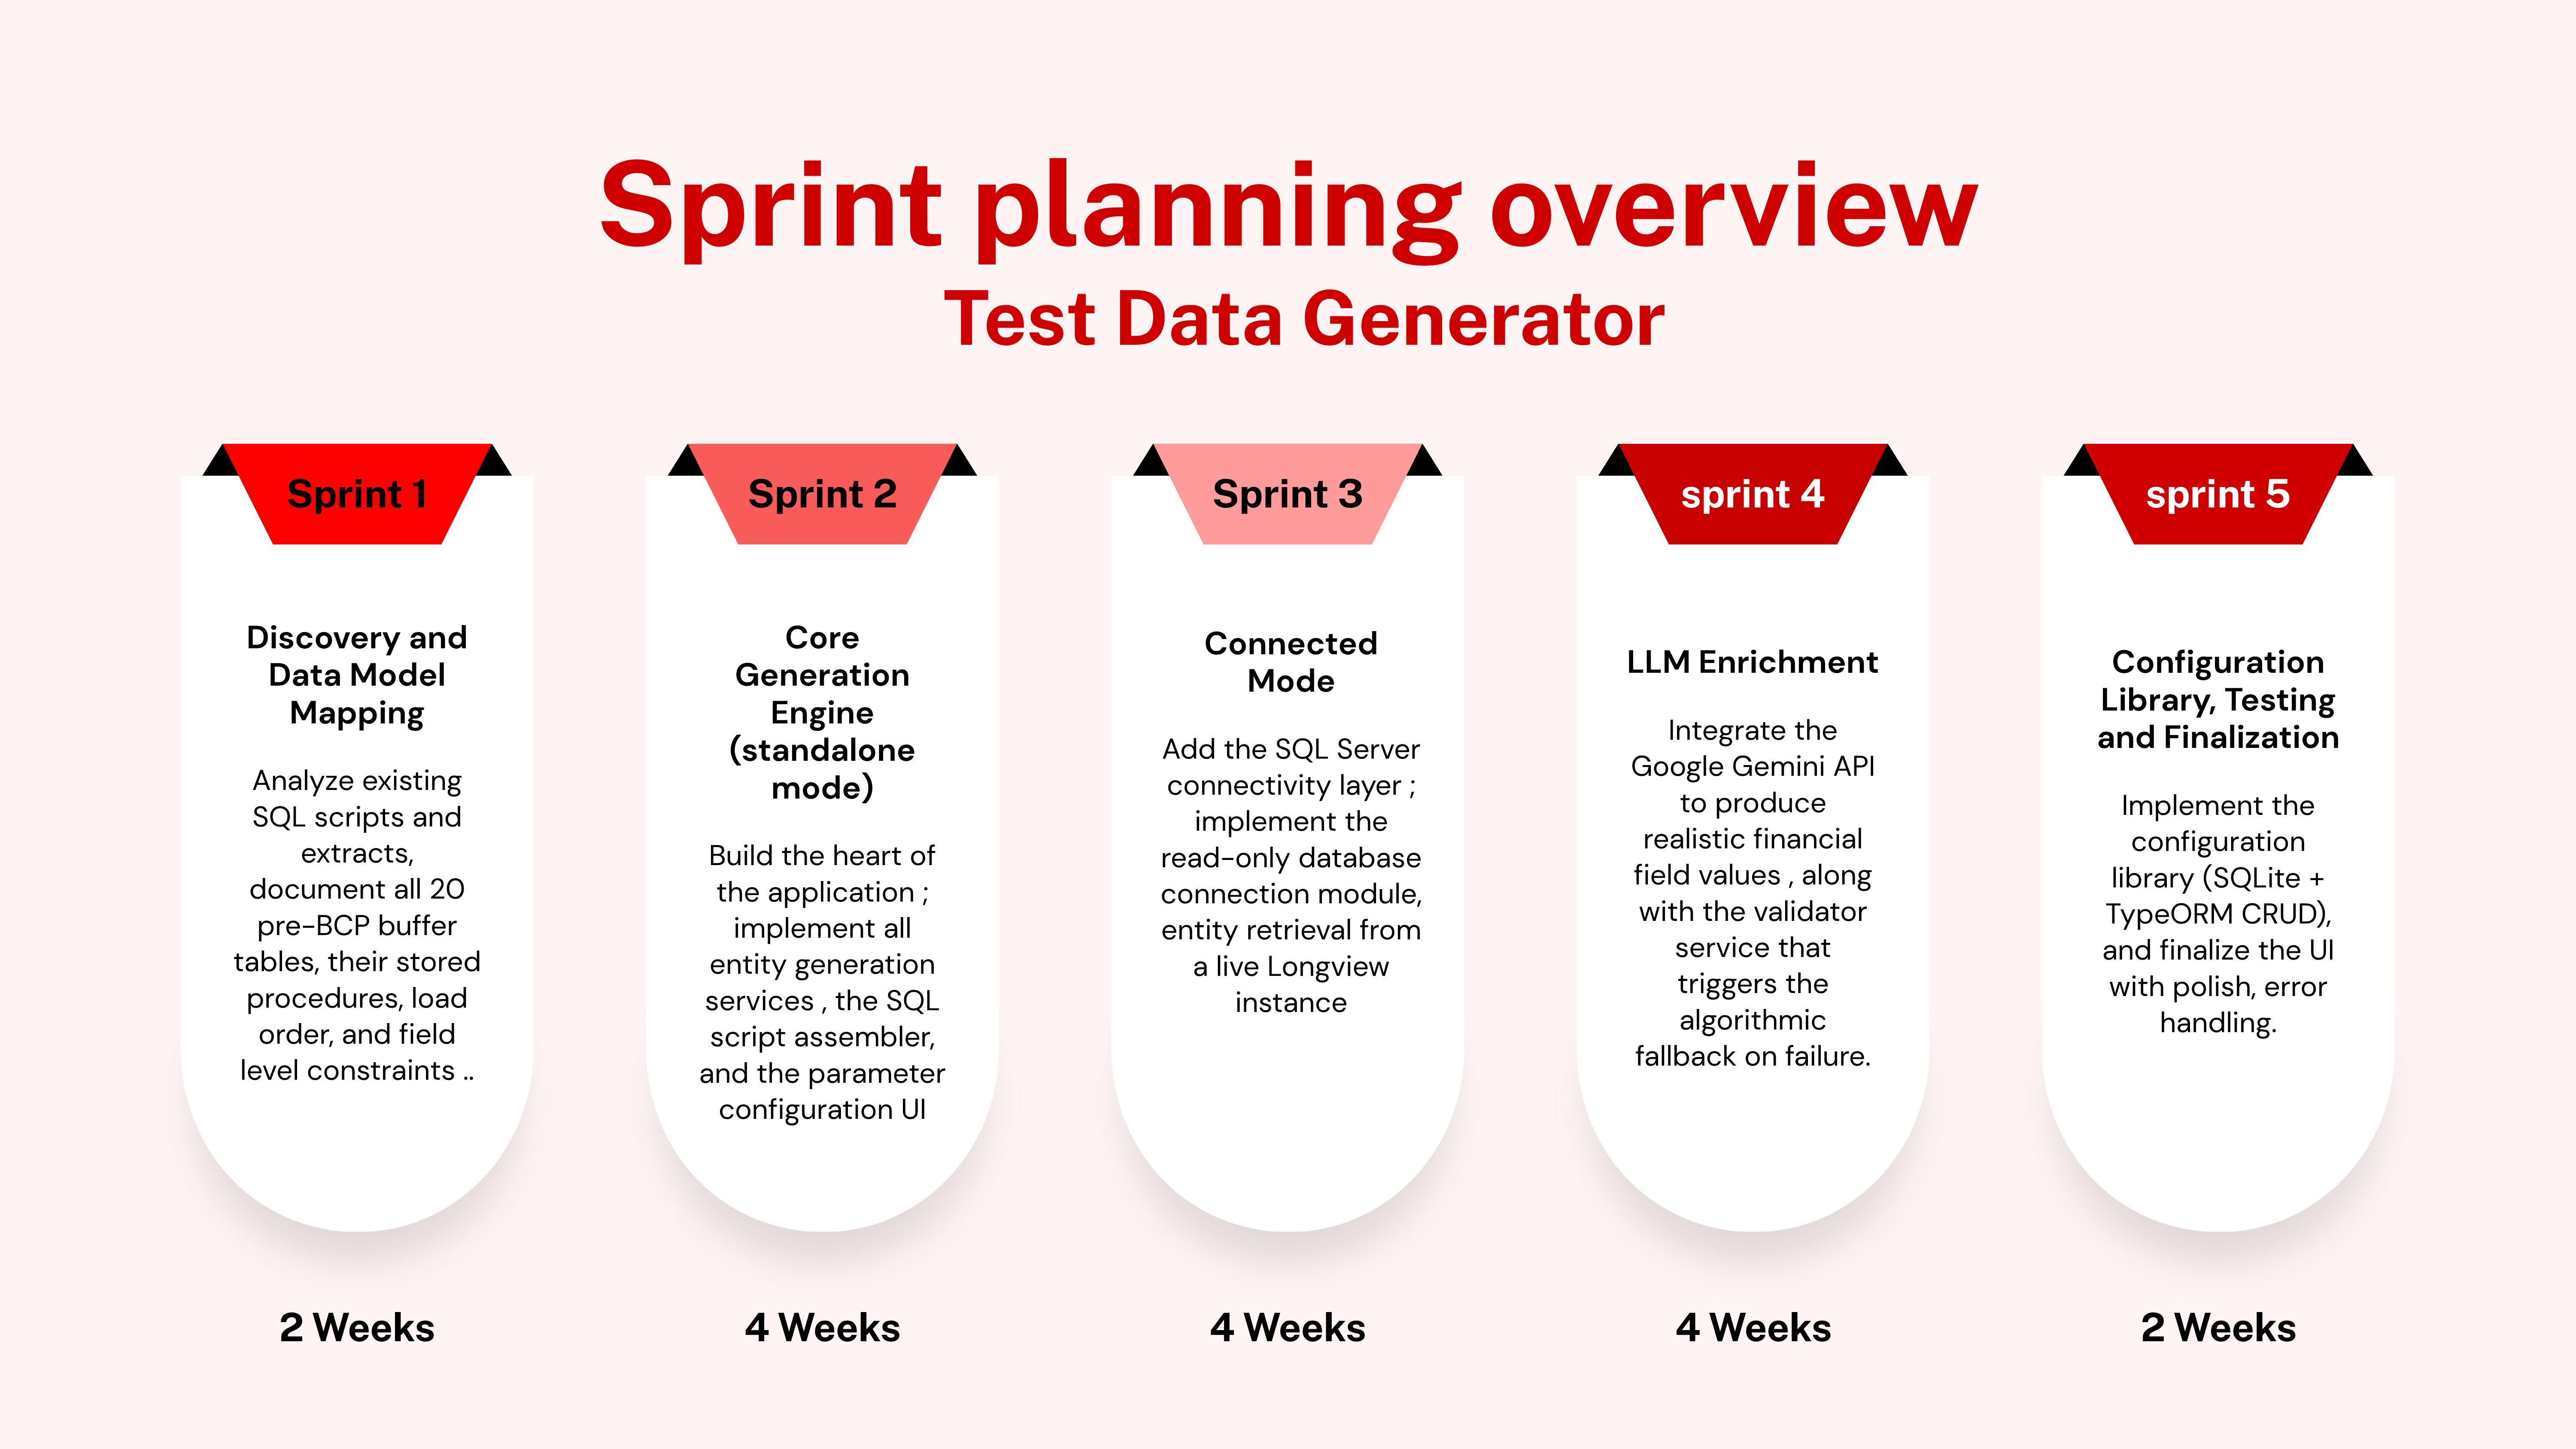
\includegraphics[width=0.95\textwidth]{img/sprint-plan.png}
\caption{Sprint planning overview}
\label{fig:sprint-plan}
\end{figure}


% ─────────────────────────────────────────────
\section{Study of Existing Solutions}
% ─────────────────────────────────────────────

\paragraph{}Before designing anything, we examined the tools and approaches
that already exist in the space of test data generation. Understanding where
they fall short in this specific context helps justify the decision to build
a custom solution.


% ─────────────────────────────────────────────
\subsection{Generic Test Data Generation Tools}
% ─────────────────────────────────────────────

\paragraph{}The most commonly used tools for generating synthetic test data
fall into three categories:

\begin{itemize}
    \item \textbf{Mockaroo} \cite{mockaroo}: A web-based tool that generates
    random data across a wide range of field types and exports it in various
    formats including SQL, CSV, and JSON. It is quick to use for simple flat
    datasets but has no concept of relational integrity or cross-table
    dependencies.

    \item \textbf{Faker} \cite{faker}: A widely
    used library available in Python, JavaScript, and other languages that
    generates plausible fake data (names, addresses, numbers, and dates).
    It is effective for populating individual fields with realistic-looking
    values, but it operates at the field level, not the dataset level.

    \item \textbf{Redgate SQL Data Generator} \cite{redgate}: This tool is
    closer to the target use case, it generates SQL \texttt{INSERT}
    statements for relational schemas and can respect foreign key
    relationships. However, it operates on a generic schema inference basis.
    It has no knowledge of financial domain rules, no concept of Longview's
    pre-BCP buffer mechanism, and no way to produce the specific Unicode
    casting and type conventions the platform requires.
\end{itemize}


% ─────────────────────────────────────────────
\subsection{Comparison Summary}
% ─────────────────────────────────────────────

\paragraph{}Table~\ref{tab:tools-comparison} summarizes how each existing
solution covers the key requirements of this project.

\begingroup
\setlength{\tabcolsep}{5pt}
\renewcommand{\arraystretch}{1.25}
\newcommand{\yes}{\textcolor{green!45!black}{\cmark}}
\newcommand{\no}{\textcolor{red!70!black}{\xmark}}
\arrayrulecolor{isiBlue!45}
\begin{longtable}{P{0.34\textwidth}
                Q{0.12\textwidth}
                Q{0.12\textwidth}
                Q{0.12\textwidth}
                Q{0.14\textwidth}}
\caption{Comparison of existing tools against project requirements}
\label{tab:tools-comparison} \\
\hline
\rowcolor{isiBlue!15}
\textbf{Criterion}
  & \textbf{Mockaroo}
  & \textbf{Faker}
  & \textbf{Redgate}
  & \textbf{Our Solution} \\
\hline
\endfirsthead
\multicolumn{5}{r}{\tablename\ \thetable{} -- \textit{continued from previous page}} \\
\hline
\rowcolor{isiBlue!15}
\textbf{Criterion}
  & \textbf{Mockaroo}
  & \textbf{Faker}
  & \textbf{Redgate}
  & \textbf{Our Solution} \\
\hline
\endhead
\hline
\multicolumn{5}{r}{\textit{continued on next page}} \\
\endfoot
\hline
\endlastfoot
\rowcolor{gray!5} Relational integrity       & \no & \no & \yes & \yes \\
Financial business rules                      & \no & \no & \no  & \yes \\
\rowcolor{gray!5} Longview SQL conventions    & \no & \no & \no  & \yes \\
LLM-enriched realism                          & \no & \no & \no  & \yes \\
\rowcolor{gray!5} Connected mode (read-only)  & \no & \no & \no  & \yes \\
No manual post-processing                     & \no & \no & \no  & \yes \\
\rowcolor{gray!5} Configuration persistence   & \no & \no & \no  & \yes \\
\hline
\end{longtable}
\arrayrulecolor{black}
\endgroup

\paragraph{}The gap these tools all share comes down to the same root cause:
they are built for the general case, not for a specific financial platform
with its own data model, its own loading conventions, and its own business
rules. This analysis confirmed that a purpose-built solution was the right
path, and that the core value of the tool lies precisely in the domain
knowledge encoded into its generation logic.


% ─────────────────────────────────────────────
\section{Requirements}
% ─────────────────────────────────────────────

% ─────────────────────────────────────────────
\subsection{Functional Requirements}
% ─────────────────────────────────────────────

\paragraph{}The functional requirements were gathered through analysis of
the existing Extracts, discussions with the Longview development and QA team,
and review of the project brief. They are organized around the two operating
modes of the system, followed by the LLM enrichment that applies to both.
The following table presents the identified functional requirements
organized by actor.

\begin{longtable}{|P{3cm}|P{10cm}|}
\caption{Description of functional requirements by actor}
\label{tab:functional-requirements} \\
\hline
\textbf{Actor} & \textbf{Functional Requirements} \\
\hline
\endfirsthead

\multicolumn{2}{r}{\tablename\ \thetable{} -- \textit{continued from previous page}} \\
\hline
\textbf{Actor} & \textbf{Functional Requirements} \\
\hline
\endhead

\hline
\multicolumn{2}{r}{\textit{continued on next page}} \\
\endfoot

\hline
\endlastfoot

QA Engineer
  & \begin{itemize}[noitemsep, topsep=2pt, leftmargin=*]
      \item Configure generation parameters (accounts, securities,
            orders, executions, positions, date ranges, asset classes)
            through a web interface
      \item Generate a complete, executable SQL script in standalone mode
            without any database connection
      \item Provide SQL Server credentials and test connectivity in
            connected mode
      \item Browse and select existing database entities (accounts,
            securities, models) to anchor generated records
      \item Trigger LLM-enriched generation for improved data realism
      \item Download the generated SQL script from the web interface
      \item Save the current generation configuration to the local
            library with a name and optional description
      \item Browse, load, rename, and delete previously saved
            configurations from the library
    \end{itemize} \\
\hline
Longview SQL Server
  & \begin{itemize}[noitemsep, topsep=2pt, leftmargin=*]
      \item Expose existing account groups, accounts, and securities
            to the system in read-only mode (connected mode only)
    \end{itemize} \\
\hline
Google Gemini API
  & \begin{itemize}[noitemsep, topsep=2pt, leftmargin=*]
      \item Receive structured prompts and return realistic financial
            field values (security names, symbols, descriptions)
      \item Trigger the algorithmic fallback transparently on
            unavailability or invalid response
    \end{itemize} \\
\hline
Local SQLite Database
  & \begin{itemize}[noitemsep, topsep=2pt, leftmargin=*]
      \item Persist named generation configurations (name,
            description, operating mode, and parameter JSON)
            across sessions in read-write mode
      \item Expose stored configurations to the backend for
            retrieval, update, and deletion via TypeORM
    \end{itemize} \\
\hline
\end{longtable}


\subsubsection{Global Use Case Diagram}

\paragraph{}Figure~\ref{fig:usecase-global} presents the global use case
diagram of the system. It summarizes the three main functional areas exposed
to the QA team: standalone generation, connected generation, and saved
configuration management. It also shows the external systems involved in the
generation process, namely the LLM API and the Longview SQL Server instance.

\begin{figure}[H]
\centering
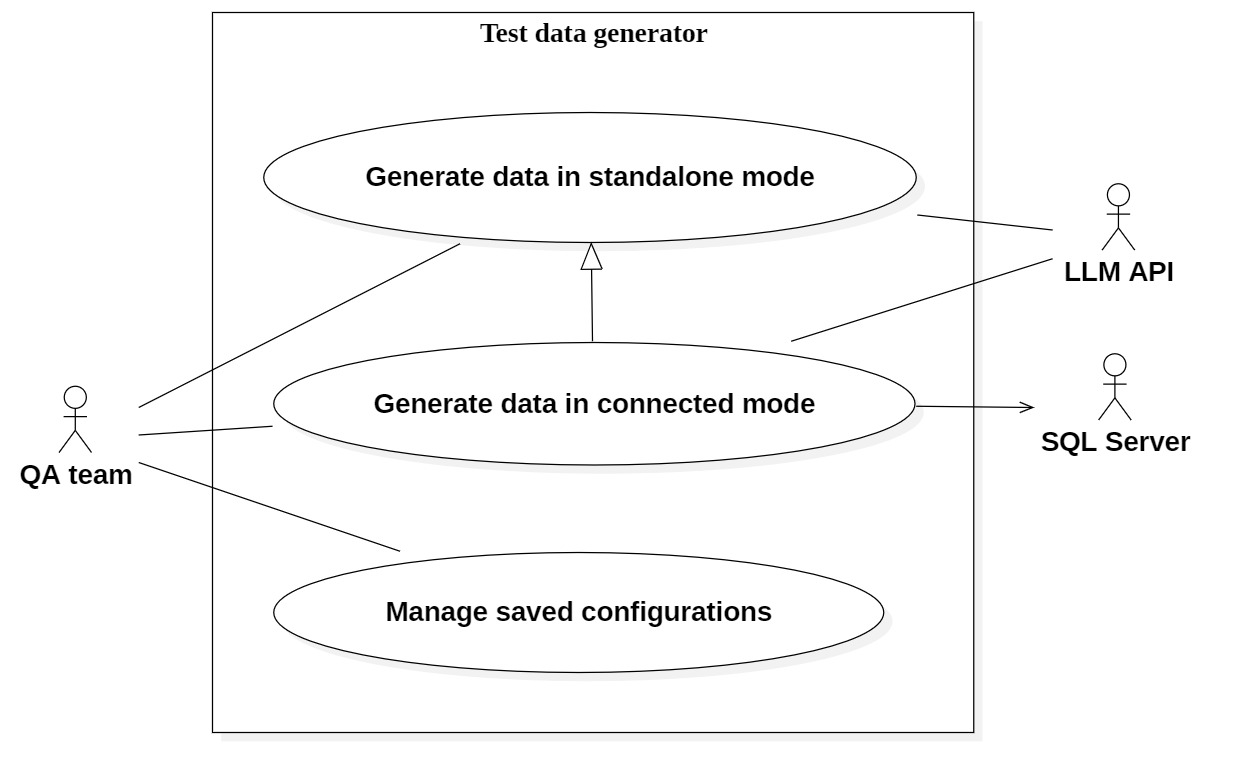
\includegraphics[width=0.9\textwidth]{img/usecase-global.jpg}
\caption{Global use case diagram of the test data generator}
\label{fig:usecase-global}
\end{figure}


% ─────────────────────────────────────────────
\subsection{Non-Functional Requirements}
% ─────────────────────────────────────────────

\paragraph{}Beyond what the system must do, the following quality
constraints shape how it must behave:

\begin{itemize}
    \item \textbf{Performance:} Generating a typical dataset -- one account
    with a full set of securities, orders, executions, and positions -- must
    complete within ten seconds in standalone mode for a typical QA dataset. LLM-assisted generation
    may take longer due to the network round-trip, but the experience must
    remain responsive from the user's perspective.

    \item \textbf{Resilience:} The system must remain fully operational
    regardless of LLM availability. If the Gemini API is unreachable or
    returns an invalid response, the algorithmic fallback must engage silently
    and complete the generation without user intervention.

    \item \textbf{Security:} The connected mode must operate in strict
    read-only mode. The application must have no capability to write, update,
    or delete data in any connected database. Connection credentials must not
    be persisted or logged beyond the active session.

    \item \textbf{Validation:} Generated datasets must be validated before
    delivery. The validator must check required fields, value formats,
    referential integrity, order and execution quantity consistency, and
    position derivation rules so that invalid records are detected before
    they reach the QA database.

    \item \textbf{Reproducibility:} A generation configuration must be
    saveable and reloadable so the same scenario can be repeated during
    regression testing. The generated output must be structured and
    inspectable, making it possible for QA engineers to archive and replay
    important scenarios.

    \item \textbf{Maintainability:} The generation logic for each entity type
    must be isolated in its own service module, so that updating a business
    rule or adding a new instrument type does not require changes across the
    entire codebase.

    \item \textbf{Extensibility:} The architecture must make it
    straightforward to add new entity types, asset classes, or output formats
    in the future without restructuring the core engine.

    \item \textbf{Usability:} The web interface must be accessible to QA
    engineers who are not necessarily developers. Error messages must be
    explicit, form inputs must be validated before submission, the generated
    SQL output must be easy to download, and frequently used parameter sets
    must be saveable and reloadable without manual re-entry.

    \item \textbf{Data Persistence:} Saved configurations must survive
    application restarts. The local SQLite database must be created
    automatically on first launch without requiring any manual installation
    or configuration from the user.
\end{itemize}


% ─────────────────────────────────────────────
\section{Global Architecture}
% ─────────────────────────────────────────────

\paragraph{}The requirements above point toward a full-stack web application
with a clear separation between the user interface, the generation logic, the
LLM integration, the database access layer, and the local configuration
persistence layer. The global package diagram is used as the logical/module
view of the solution, while the physical architecture diagram focuses on where
the main runtime elements are deployed and how they communicate.


% ─────────────────────────────────────────────
\subsection{Global Package Diagram}

\paragraph{}Figure~\ref{fig:global-package-diagram} presents the global package diagram of the application.
It serves as the logical organization view of the system. It shows how the frontend modes,
backend API, generation services, configuration library, LLM enrichment layer, and database
access services are organized and how they collaborate around the generated dataset and saved
configurations.

\begin{figure}[H]
\centering
\makebox[\textwidth][c]{%
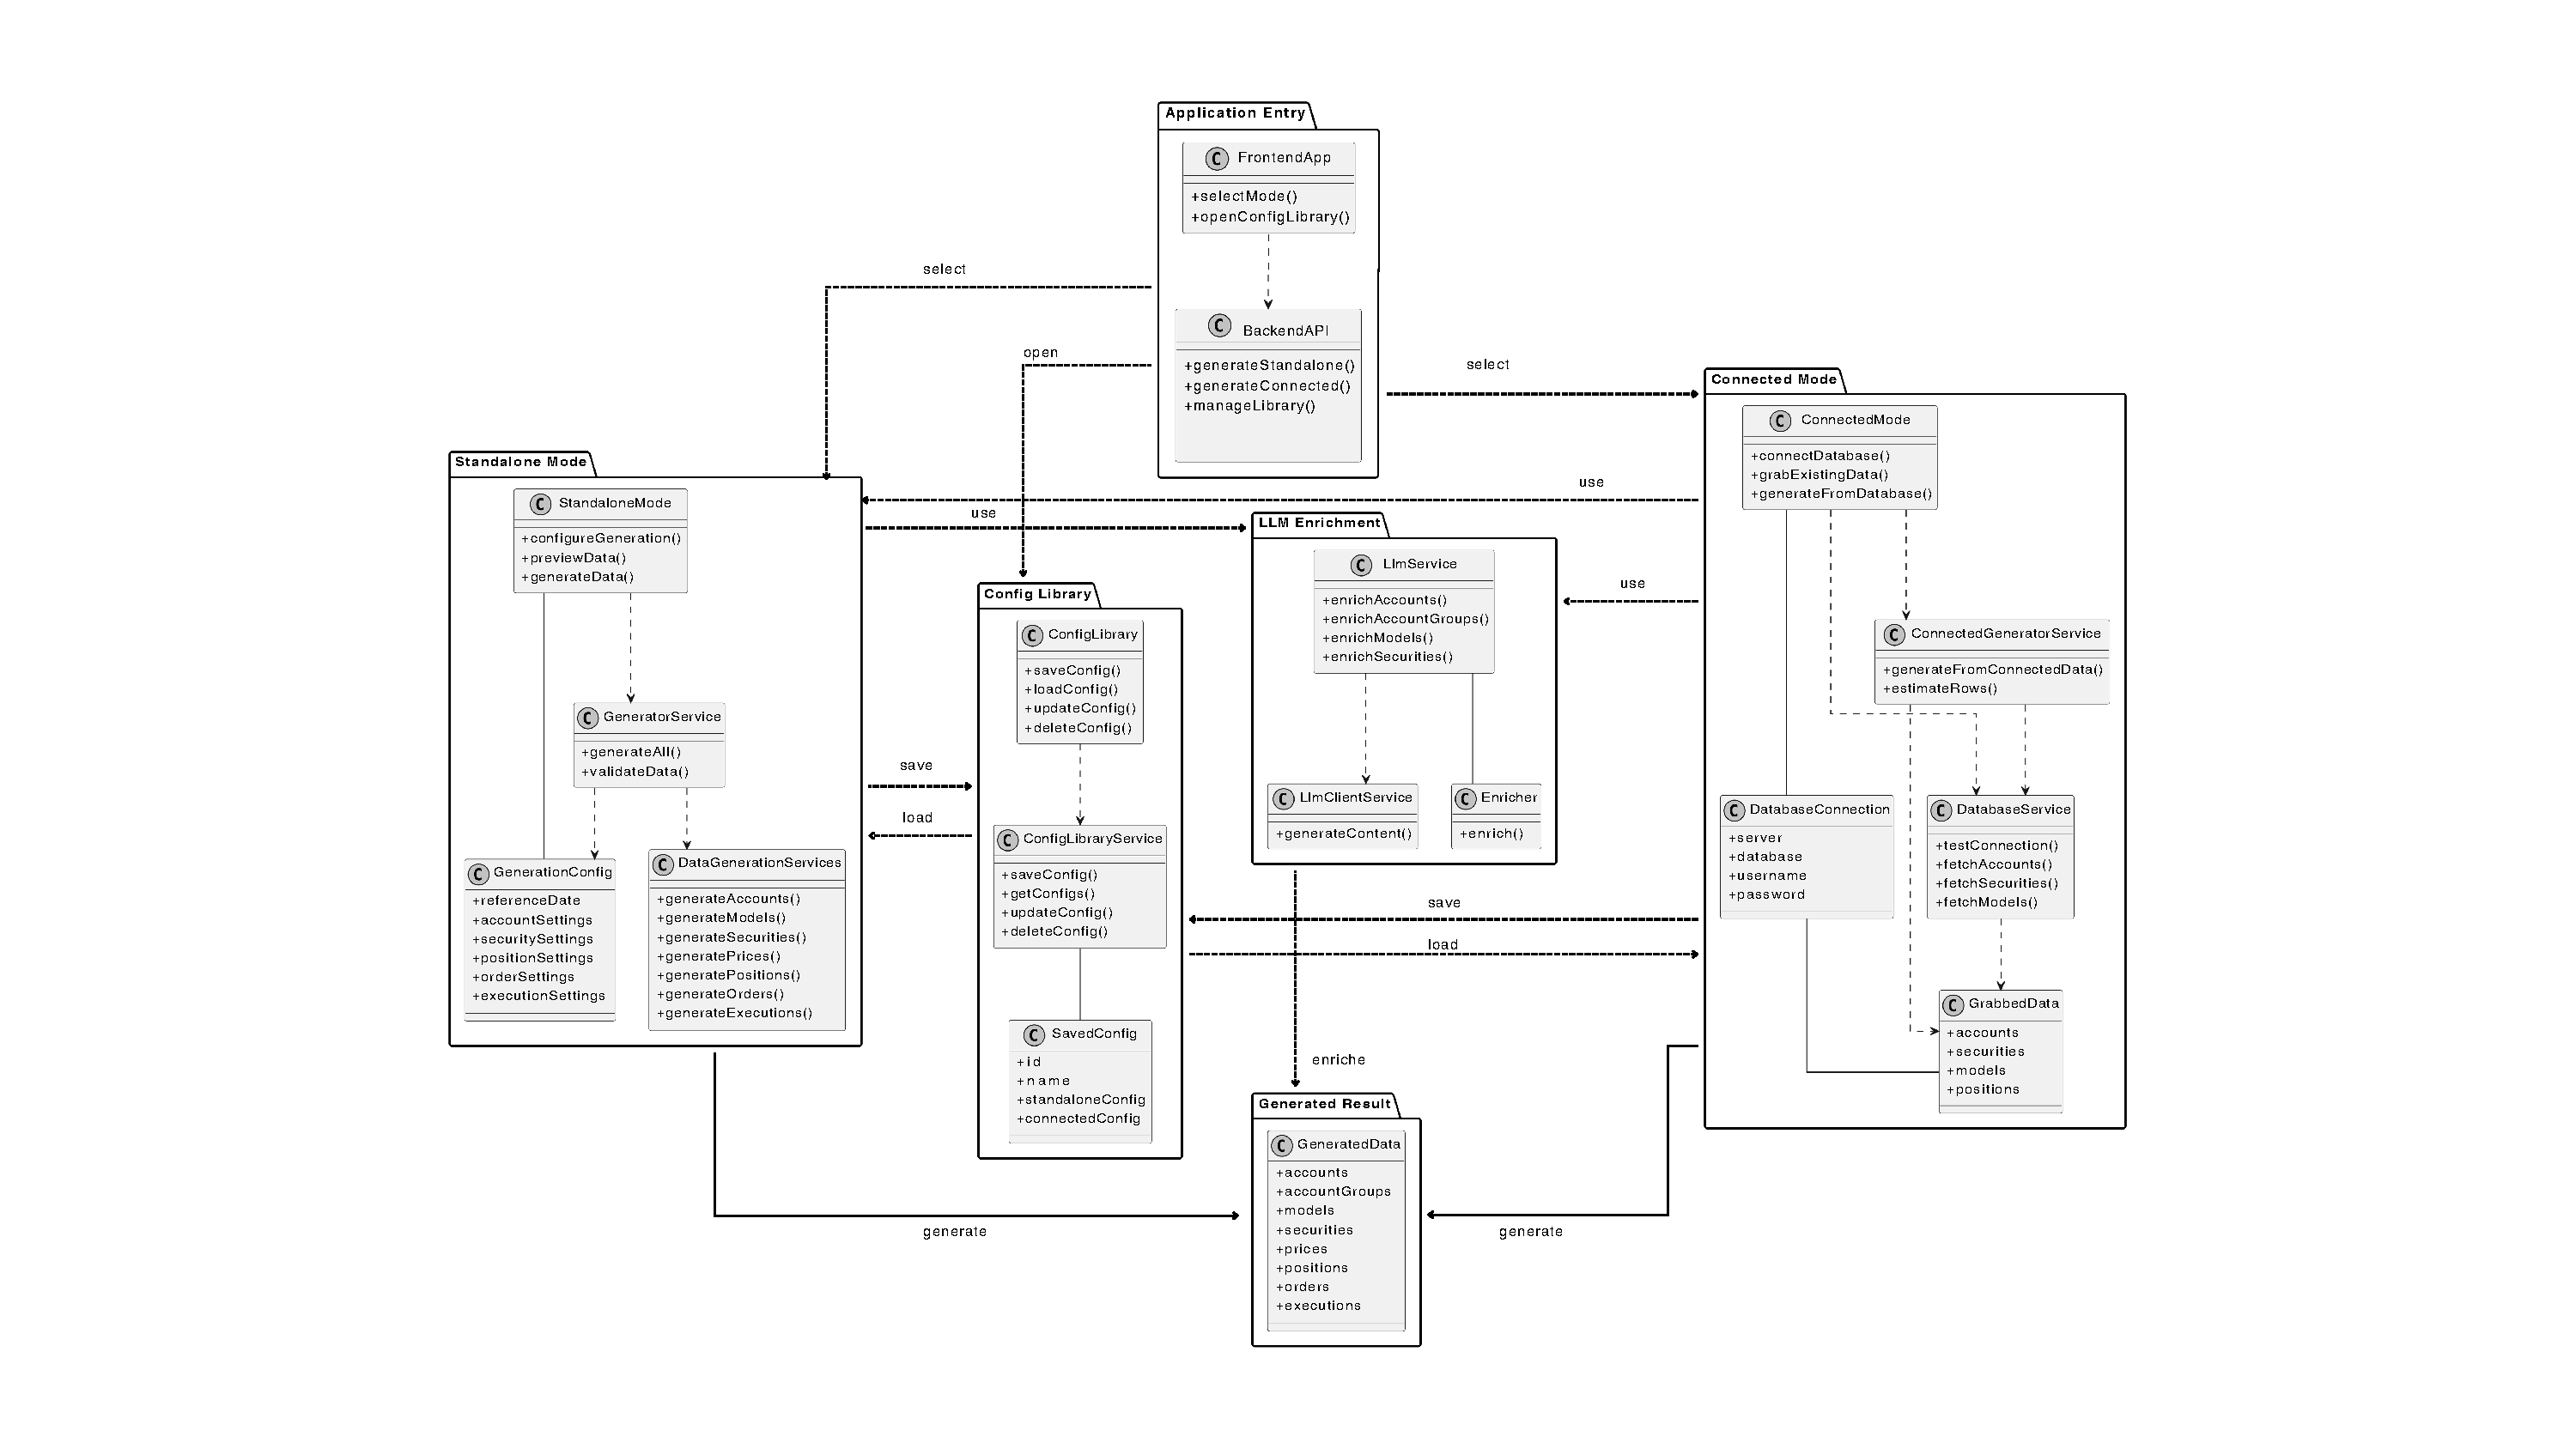
\includegraphics[width=1.4\textwidth,height=0.92\textheight,keepaspectratio]{img/global-package-diagram.pdf}}
\caption{Global package diagram of the test data generator}
\label{fig:global-package-diagram}
\end{figure}


% ─────────────────────────────────────────────

% ─────────────────────────────────────────────
\subsection{Physical Architecture}
% ─────────────────────────────────────────────

\paragraph{}Figure~\ref{fig:arch-physical} presents the physical architecture of the
application. Unlike the package diagram, which explains the internal software
organization, this view shows the deployed runtime elements and the external
systems used by the application.

\begin{itemize}
    \item The \textbf{web browser} is used by the QA team to access the React
    interface.
    \item The \textbf{frontend application} is served as a React/Vite web
    application and communicates with the backend through REST/JSON requests.
    \item The \textbf{NestJS backend} runs as a Node.js REST API and hosts the
    generation, connected mode, configuration library, LLM, and SQL script
    generation modules.
    \item The \textbf{SQLite database} (\texttt{config-library.db}) is a local
    file used to persist saved configurations.
    \item The \textbf{SQL Server database} is an external Longview database
    accessed only in connected mode and only for read operations.
    \item The \textbf{Gemini API} is an external cloud service used for LLM
    enrichment when it is enabled.
    \item The \textbf{output directory} stores the generated DAT files and the
    final SQL loading script.
\end{itemize}

\begin{figure}[H]
\centering
\makebox[\textwidth][c]{%
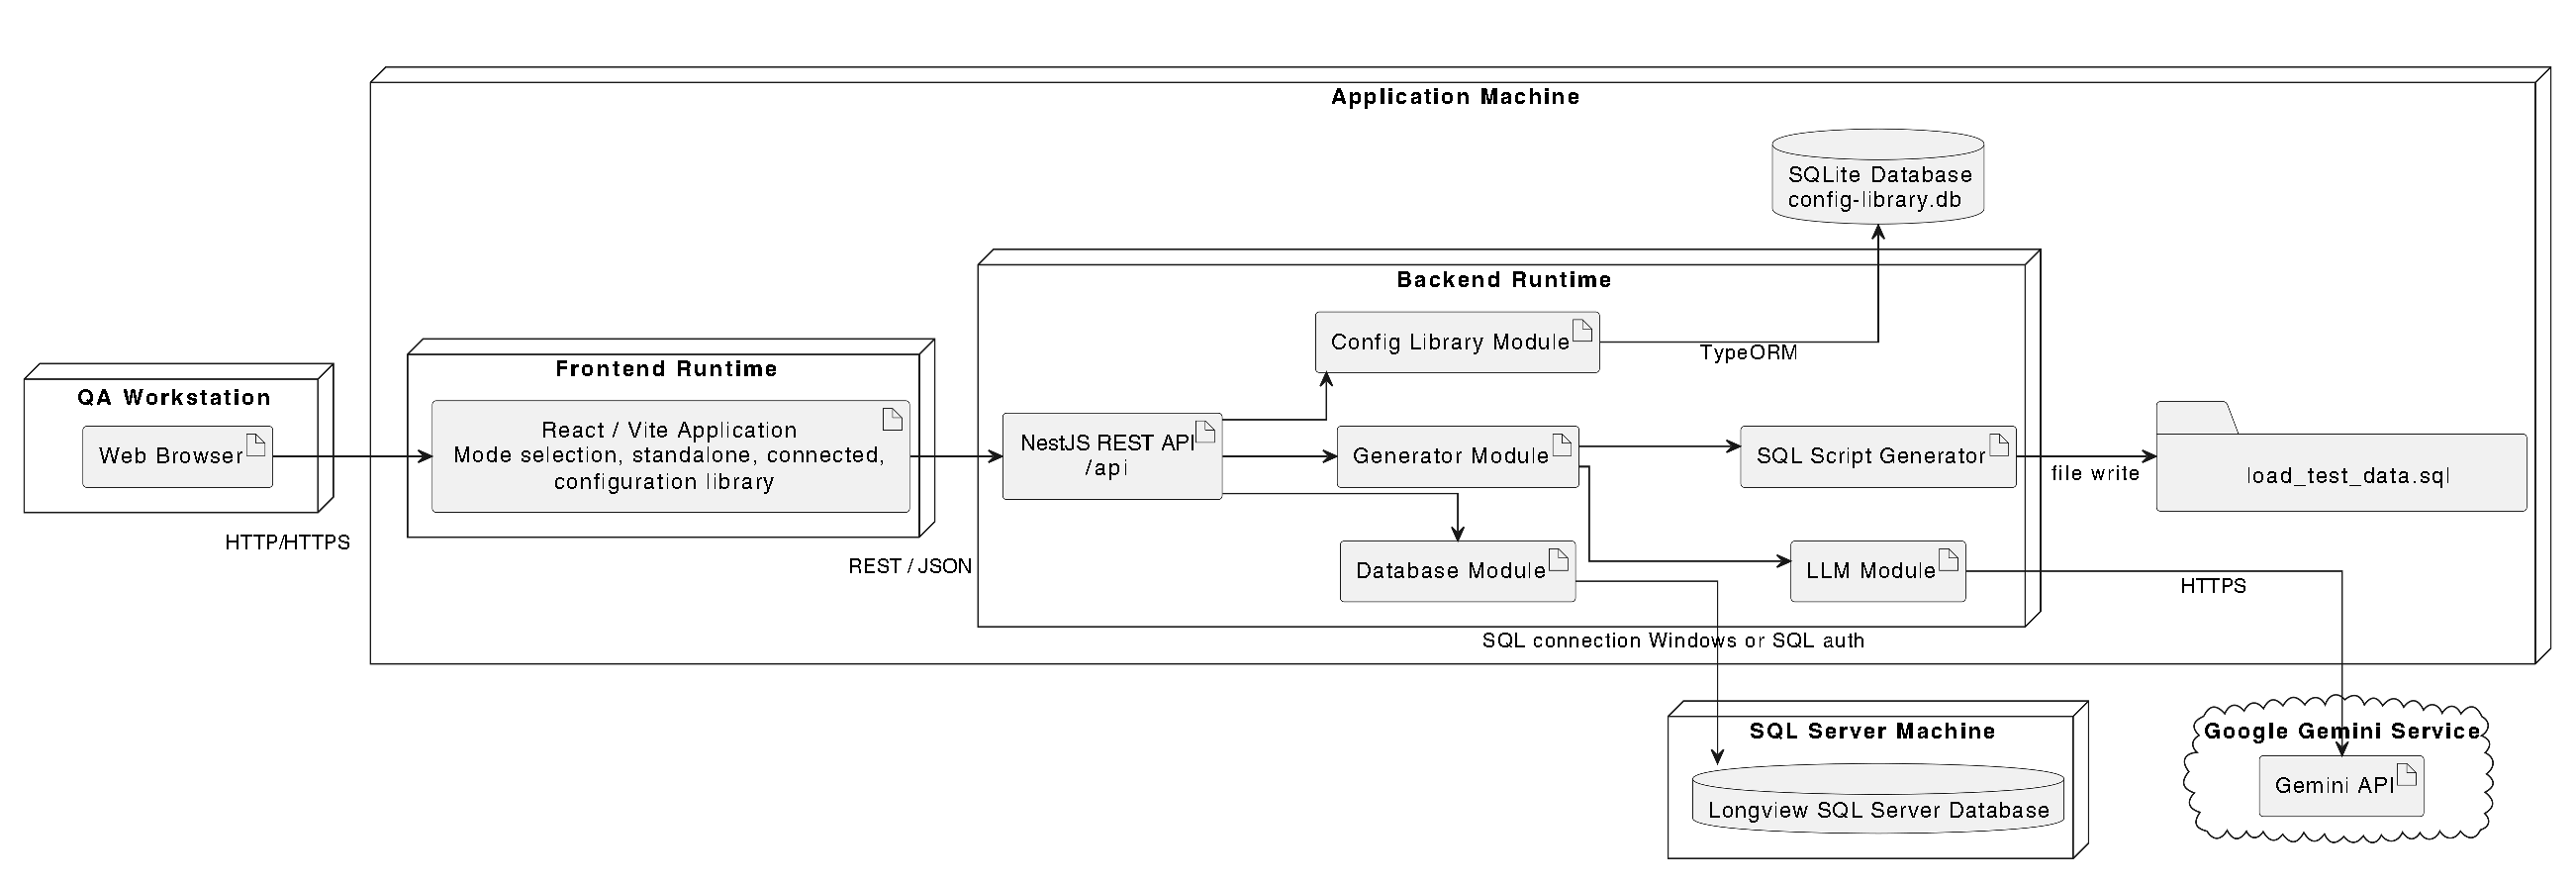
\includegraphics[width=1\textwidth,height=0.84\textheight,keepaspectratio]{img/arch-physical.pdf}}
\caption{Physical architecture of the test data generator}
\label{fig:arch-physical}
\end{figure}


% ─────────────────────────────────────────────
\section{Product Backlog and Sprint Planning}
% ─────────────────────────────────────────────

\paragraph{}The product backlog captures all user stories identified during
the analysis phase, prioritized in collaboration with the Product Owner.
Each user story is expressed from the perspective of the QA engineer or the
system actor that benefits from it. The detailed breakdown of tasks for each
story is presented at the beginning of the corresponding sprint chapter.
Table~\ref{tab:backlog} presents the global product backlog.

\begin{longtable}{|Q{0.08\textwidth}|P{4cm}|P{8.5cm}|}
\caption{Product backlog}
\label{tab:backlog} \\
\hline
\textbf{ID} & \textbf{User Story} & \textbf{Description} \\
\hline
\endfirsthead

\multicolumn{3}{r}{\tablename\ \thetable{} -- \textit{continued from previous page}} \\
\hline
\textbf{ID} & \textbf{User Story} & \textbf{Description} \\
\hline
\endhead

\hline
\multicolumn{3}{r}{\textit{continued on next page}} \\
\endfoot

\hline
\endlastfoot

1 & Generation Parameter Configuration
  & As a QA engineer, I want to configure generation parameters through
    a web form so that I can control entity types, counts, date ranges,
    and operating mode without editing any file. \\
\hline
2 & Account and Account Group Generation
  & As a QA engineer, I want to generate accounts, account groups, and
    hierarchy records so that I can test the full account structure
    loading pipeline. \\
\hline
3 & Model Generation
  & As a QA engineer, I want to generate investment model and
    model-objective records so that I can test model-driven
    allocation scenarios. \\
\hline
4 & Equity and Generic Security Generation
  & As a QA engineer, I want to generate equity and generic instrument
    records so that I can test the loading of basic security types. \\
\hline
5 & Fixed Income Security Generation
  & As a QA engineer, I want to generate fixed income securities along
    with their call, put, coupon, and convertible schedules so that I
    can test the full bond loading pipeline. \\
\hline
6 & Derivative Security Generation
  & As a QA engineer, I want to generate options, futures, and FX
    forward records so that I can test the loading of derivative
    instruments. \\
\hline
7 & Price Generation
  & As a QA engineer, I want to generate price records consistent with
    the generated securities so that I can test the pricing
    load pipeline. \\
\hline
8 & Order and Execution Generation
  & As a QA engineer, I want to generate proposed orders and execution
    records anchored to existing securities and accounts so that I can
    test the full order lifecycle pipeline. \\
\hline
9 & Position Generation
  & As a QA engineer, I want to generate tax-lot position records
    consistent with executed orders so that I can test the position
    loading pipeline. \\
\hline
10 & SQL Script Assembly and Download
  & As a QA engineer, I want the system to assemble and deliver a
    complete, executable SQL script so that I can load all generated
    data into Longview with a single file. \\
\hline
11 & Connected Mode
  & As a QA engineer, I want to connect to a live Longview instance
    in read-only mode so that I can anchor generated records to
    existing database entities. \\
\hline
12 & LLM Enrichment
  & As a QA engineer, I want to enable AI-assisted generation so that
    security names, ticker symbols, and descriptions are realistic
    and contextually meaningful. \\
\hline
13 & Configuration Library
  & As a QA engineer, I want to save and reload named generation
    configurations so that I do not have to re-enter parameters at
    every session. \\
\hline
14 & Validation and Error Handling
  & As a QA engineer, I want the interface to validate my inputs and
    display clear error messages so that I can correct mistakes before
    triggering generation. \\
\hline

\end{longtable}

\paragraph{}The 14 user stories are distributed across five sprints as
shown in Figure~\ref{fig:sprint-plan}. The detailed task breakdown for each
sprint is presented at the beginning of the corresponding implementation
chapter.


% ─────────────────────────────────────────────
\section{Technical Environment}
% ─────────────────────────────────────────────

\paragraph{}The technology choices reflect both the system requirements and
the constraints of the internship environment, covering the full development
chain from the user interface down to the database layer.


% ─────────────────────────────────────────────
\subsection{Hardware}
% ─────────────────────────────────────────────

\paragraph{}Development was carried out on a standard workstation provided
by Linedata Tunisia, running Windows 11. The machine hosted both the
frontend and backend development servers locally and provided connectivity
to the SQL Server instances available in the team's development environment.


% ─────────────────────────────────────────────
\subsection{Software and Technologies}
% ─────────────────────────────────────────────

\paragraph{}In this project, we used the following technologies and tools:


% ── React ──────────────────────────────────────
\paragraph{}\textbf{React 18 + TypeScript}\\
React is an open-source JavaScript library for building user interfaces
through reusable components. Combined with TypeScript, it provides strong
static typing that reduces runtime errors and improves code maintainability.
React was chosen for the frontend of this project due to its component-based
architecture and its suitability for building form-heavy, interactive
interfaces such as the generation parameter configuration panel.
\begin{figure}[H]
\centering

\includegraphics[width=0.12\textwidth]{img/logo-react.png}
\caption{React logo}
\label{fig:logo-react}
\end{figure}


% ── Tailwind CSS ───────────────────────────────
\paragraph{}\textbf{Tailwind CSS + shadcn/ui}\\
Tailwind CSS is a utility-first CSS framework that enables rapid and
consistent UI development directly in markup, without writing custom
stylesheets. It was complemented by shadcn/ui, a collection of accessible
and composable UI components built on top of Radix UI primitives, which
provided ready-made form controls, dialogs, and layout elements consistent
with the application's design system.
\begin{figure}[H]
\centering

\includegraphics[width=0.12\textwidth]{img/logo-tailwind.png}
\caption{Tailwind CSS logo}
\label{fig:logo-tailwind}
\end{figure}


% ── Vite ───────────────────────────────────────
\paragraph{}\textbf{Vite}\\
Vite is a modern frontend build tool that provides an extremely fast
development server through native ES module support, as well as optimized
production builds. It was selected as the build tool for the React frontend
due to its near-instant cold start and hot module replacement, which
significantly improved the development experience.
\begin{figure}[H]
\centering

\includegraphics[width=0.12\textwidth]{img/logo-vite.png}
\caption{Vite logo}
\label{fig:logo-vite}
\end{figure}


% ── NestJS ─────────────────────────────────────
\paragraph{}\textbf{NestJS + TypeScript}\\
NestJS is a progressive Node.js framework for building efficient and
scalable server-side applications. Its modular, decorator-based architecture
maps naturally to the service-per-entity design of the generation engine,
where each entity type (securities, accounts, orders, executions, positions)
is encapsulated in its own dedicated service module. TypeScript support is
first-class and shares the same type definitions with the frontend.
\begin{figure}[H]
\centering

\includegraphics[width=0.12\textwidth]{img/logo-nestjs.png}
\caption{NestJS logo}
\label{fig:logo-nestjs}
\end{figure}


% ── Node.js ────────────────────────────────────
\paragraph{}\textbf{Node.js}\\
Node.js is an open-source, cross-platform JavaScript runtime environment
that executes JavaScript code outside of a browser, on the server side.
It serves as the runtime underlying the NestJS backend, enabling
non-blocking I/O operations that are well-suited for handling concurrent
API requests during generation.
\begin{figure}[H]
\centering

\includegraphics[width=0.12\textwidth]{img/logo-nodejs.png}
\caption{Node.js logo}
\label{fig:logo-nodejs}
\end{figure}


% ── SQL Server ─────────────────────────────────
\paragraph{}\textbf{Microsoft SQL Server + node-mssql}\\
Microsoft SQL Server is the relational database management system underlying
all Longview deployments. It is the target platform for the generated SQL
scripts. The \texttt{node-mssql} package was used as the Node.js driver to
establish the read-only connection in connected mode, offering connection
pooling and parameterized query support.
\begin{figure}[H]
\centering

\includegraphics[width=0.12\textwidth]{img/logo-sqlserver.png}
\caption{Microsoft SQL Server logo}
\label{fig:logo-sqlserver}
\end{figure}


% ── TypeORM + SQLite ───────────────────────────
\paragraph{}\textbf{TypeORM + SQLite (better-sqlite3)}\\
TypeORM is an object-relational mapper for TypeScript and Node.js that
supports multiple database drivers and integrates natively with NestJS
through decorator-based entity definitions. It was used to manage the
\texttt{SavedConfig} entity with automatic schema synchronization, which
eliminates the need for manual migration scripts in the development context.
The \texttt{better-sqlite3} driver was selected as the underlying database
    engine because SQLite is self-contained and serverless -- the database is
stored as a single local file (\texttt{config-library.db}) that TypeORM
creates automatically on first startup, requiring zero infrastructure from
the user.
\begin{figure}[H]
\centering

\includegraphics[width=0.12\textwidth]{img/logo-typeorm.png}
\caption{TypeORM logo}
\label{fig:logo-typeorm}
\end{figure}


% ── Gemini API ─────────────────────────────────
\paragraph{}\textbf{Google Gemini API}\\
Google Gemini is a family of large language models developed by Google
DeepMind. Its REST API was integrated as the LLM enrichment layer of the
generation engine, tasked with producing realistic security names, ticker
symbols, and financial descriptions from structured prompts. An algorithmic
fallback ensures the system remains fully functional when the API is
unavailable.
\begin{figure}[H]
\centering

\includegraphics[width=0.12\textwidth]{img/logo-gemini.png}
\caption{Google Gemini API logo}
\label{fig:logo-gemini}
\end{figure}


% ── Git + GitHub ───────────────────────────────
\paragraph{}\textbf{Git + GitHub}\\
Git is the standard distributed version control system used to track all
changes across the project. GitHub was used as the remote repository
host, enabling branch management, commit history tracking, and sprint-level
progress visibility throughout the internship.
\begin{figure}[H]
\centering

\includegraphics[width=0.12\textwidth]{img/logo-github.png}
\caption{GitHub logo}
\label{fig:logo-github}
\end{figure}


% ── VS Code ────────────────────────────────────
\paragraph{}\textbf{Visual Studio Code}\\
Visual Studio Code is a lightweight and highly extensible source-code
editor developed by Microsoft. It was used as the primary IDE throughout
the project, leveraging extensions for TypeScript IntelliSense, NestJS
snippets, ESLint, Prettier, and the REST Client for API testing directly
within the editor.
\begin{figure}[H]
\centering

\includegraphics[width=0.12\textwidth]{img/logo-vscode.png}
\caption{Visual Studio Code logo}
\label{fig:logo-vscode}
\end{figure}


% ─────────────────────────────────────────────
\section*{Conclusion}
\addcontentsline{toc}{section}{Conclusion}
% ─────────────────────────────────────────────

\paragraph{}This chapter covered the full analysis and design process that
laid the foundation of the project. We adopted Scrum as the development
framework and organized the work into five incremental sprints. A review of
existing test data generation tools confirmed that none of them could address
the specificity of the Longview context, validating the need for a
purpose-built solution. From the functional and non-functional requirements,
we derived a layered architecture built around a React frontend, a NestJS
backend with entity-specific generation services, a Gemini API integration
for data realism, a read-only SQL Server connection for connected mode, and
a local SQLite persistence layer that allows QA engineers to save and reload
named generation configurations across sessions. This design was documented
through a global use case diagram, a global package diagram, and a physical
architecture diagram, each covering a distinct view of the system. The 14 user stories
organized in the product backlog and distributed across five sprints gave
the implementation a clear and structured roadmap. The next chapter covers
Sprint 1, the discovery phase in which the existing SQL scripts were analyzed
and the Longview data model was fully mapped in preparation for the
generation engine.
